\subsection{AIM-120 AMRAAM}
\label{subsec:aim120}
\begin{figure}[htbp]
    \centering
    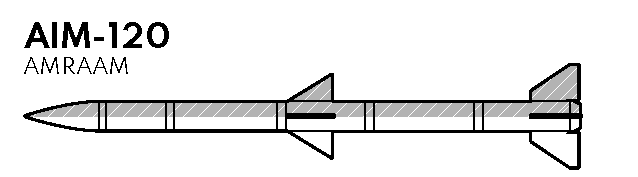
\includegraphics[
            width = 108mm,
    ]{F16_aaweapons_amraam_overview_v01.pdf}
    \fbox{
    \begin{minipage}[t][25mm][t]{100mm}
        \center{\large\textbf{AIM-120 OVERVIEW}}
        \begin{itemize}
            \item Some kind of overview figure
        \end{itemize}
    \end{minipage}
    }
    \caption{AIM-120 AMRAAM}
\end{figure}

\begin{tcoloritemize}
    \blueitem{AIM-120 \break AMRAAM}{
    \textbf{A}dvanced \textbf{M}edium \textbf{R}ange \textbf{A}ir-to-\textbf{A}ir \textbf{M}issile
    --- long range, fire-and-forget, active-radar homing missile

    \begin{subitemize}
        \item \textbf{Guidance} --- Active Radar-Guided (\textbf{Fox 3})
        \item \textbf{Range} --- max:  \textasciitilde30-40nm (high mach, alt)
    \end{subitemize}}
    \blueitem{Employment \break Types}{
    \begin{subitemize}
        \item \textbf{Maddog / Active Launch  (no radar)} \\
        \hyperref[subsec:aim120:maddog]{See \Cref{subsec:aim120:maddog}}
        \item \textbf{Single-target employment (STT lock or TWS/DTT bug)}
        \hyperref[subsec:aim120:single]{See \Cref{subsec:aim120:single}}
        \item \textbf{Multi-target employment (TWS/DTT bug)} \\
        \hyperref[subsec:aim120:multi]{See \Cref{subsec:aim120:multi}}
    \end{subitemize}}
    \blueitem{Flight Profile}{Successful long-range weapon employment necessitates understanding of flight-profile and tactics
    \begin{subitemize}
        \item \textbf{Mid-Course} --- Guided via \underline{datalink}, launching fighter should maintain radar contact with target
        \item \textbf{Terminal Phase} --- Guided via \underline{internal radar}, launching fighter may break away
    \end{subitemize}
    
    \textbf{See \Cref{subsec:bvr} and \Cref{subsec:bvr:tacticalconsideration}}
    }
    \blueitem{Select AIM-120}{
    Via A-A Master Mode

    \begin{subenumerate}
        \item \textbf{Master Mode} \dotfill \textbf{A-A}
        \item \textbf{Operating Mode (SMS OSB 1)} \dotfill Verify \textbf{AAM}
        \item \textbf{Selected Weapon (SMS OSB 7)} \dotfill \textbf{120C}
    \end{subenumerate}

    Via Missile Override

    \begin{subenumerate}
        \item \textbf{DGFT/MSL OVRD} \dotfill \textbf{OVRD}
        \item \textbf{Selected Weapon (SMS OSB 7)} \dotfill \textbf{120C} 
    \end{subenumerate}
    
    Via Dogfight

    \begin{subenumerate}
        \item \textbf{DGFT/MSL OVRD} \dotfill \textbf{DGFT}
        \item \textbf{Selected Weapon (SMS OSB 7)} \dotfill \textbf{120C}
    \end{subenumerate}
    
    Selected weapon can also be cycled with \textbf{NWS/MSL Step depress (long)}
    }
\end{tcoloritemize}

\subsubsection{SMS CONTROLS}
\label{subsec:aim120:sms}
\begin{tcoloritemize}
    \blueitem{Selected Weapon}{
    \textbf{OSB 7} cycles through available A-A weapon types
    
    \medskip
    Selected weapon can also be cycled with \textbf{NWS/MSL Step depress (long)}
    }
    \blueitem{Selected Station}{
    \textbf{OSB 10 / 16} select/cycle availabel missile pylons
    
    \medskip
    Selected station can also be cycled with \textbf{NWS/MSL Step depress (short)}
    }
    \blueitem{SLAVE / BORE}{\textbf{OSB 19} controls missile radar line-of-sight
    \begin{subitemize}
        \item \textbf{SLAVE} --- Missile LOS slaved to AC radar 
        \begin{itemize}
            \item receives DL updates until within own radar limits
        \end{itemize}
        \item \textbf{BORE} --- Missile scans straight ahead
        \begin{itemize}
            \item tracks first detected target
        \end{itemize}
    \end{subitemize}
    
    Line-of-sight mode can also be cycled with \textbf{Cursor Enable Depress}}
\end{tcoloritemize}

\begin{figure}[htbp]
    \centering
    \begin{tikzpicture}[auto, node distance=10mm, x=1mm, y=1mm, very thick, line cap=round,
        >={Latex[round]}
        ]
        
        \node[] (fig) at (0,0) {
            \includegraphics[
                height=75mm,
                page={7},
            ]{F16_aaweapons_missilelaunch_new_v2.pdf}
        };

        % Annotations
        \node[lannot] (mode) at ($(fig.west)+(-2.5mm,27mm)$) {Operating \\ mode};
        \draw[->, red] (mode.east) -- ++(15mm, 0mm) -- (-24mm,32mm);

        \node[lannot] (los) at ($(fig.west)+(-2.5mm,14.25mm)$) {LOS mode};
        \draw[->, red] (los.east) -- ++(5mm, 0mm);

        \node[lannot] (lstation) at ($(fig.west)+(-2.5mm,-23mm)$) {Selected station};
        \draw[->, red] (lstation.east) -- ++(5mm, 0mm);

        \node[rannot] (inv) at ($(fig.east)+(2.5mm,27mm)$) {Inventory};
        \draw[->, red] (inv.west) -- ++(-26mm, 0mm) -- (13mm, 32mm);

        \node[rannot] (sel) at ($(fig.east)+(2.5mm,14.25mm)$) {Selected \\ weapon};
        \draw[->, red] (sel.west) -- ++(-5mm, 0mm);

        \node[rannot] (lstation) at ($(fig.east)+(2.5mm,-23mm)$) {Selected station};
        \draw[->, red] (lstation.west) -- ++(-5mm, 0mm);

        \node[rannot] (sj) at ($(fig.east)+(2.5mm,-40mm)$) {Selective Jettison};
        \draw[->, red] (sj.west) -- ++(-15mm, 0mm) -- ($(fig.south) + (25mm,2mm)$);
    \end{tikzpicture}
    \caption{AIM-120 SMS page}
\end{figure}

\clearpage

\subsubsection{SYMBOLOGY}
\label{subsec:aim120:symb}

\begin{tcoloritemize}
    \blueitem{Basic Radar Symbology}{For beyond-visual-range radar usage and symbology \textbf{reference \Crefrange{subsec:crm}{subsec:tws}}}
    \blueitem{DLZ}{\textbf{D}ynamic \textbf{L}aunch \textbf{Z}one
    \begin{subitemize}
        \item \textbf{Displays target range \& missile performance information on HUD \& FCR Page with}
        \begin{itemize}
            \item missile selected
            \item radar track acquired
        \end{itemize}
        \item \textbf{R\textsubscript{aero} --- Aerodynamic range}
        \begin{itemize}
            \item \underline{maximum kinetic range}
            \item assumes non-maneuvering target
        \end{itemize}
        \item \textbf{R\textsubscript{opt} --- Optimal}
        \item \textbf{R\textsubscript{PI} --- Probability Intercept}
        \item \textbf{R\textsubscript{TR} --- Turn-and-run range}
        \begin{itemize}
            \item maximum range assuming target turns cold at current velocity
        \end{itemize}
        \item \textbf{R\textsubscript{ACT} --- Active range}
        \begin{itemize}
            \item range at which AIM-120 will go active
            \item not shown in \ref{fig:aa_weap:aim120:dlz}
        \end{itemize}
        \item \textbf{R\textsubscript{MIN} --- Minimum range}
        \item \textbf{Countdown}
        \begin{itemize}
            \item \textbf{A} --- seconds until missile goes active
            \item \textbf{T} --- seconds until predicted impact
        \end{itemize}
    \end{subitemize}
    Reference \cref{fig:aa_weap:aim120:dlz}}
    \blueitem{ASC \& ASEC}{
    \begin{subitemize}
        \item \textbf{Displays target lead cues to maximize missile performance on HUD \& FCR Page with}
        \begin{itemize}
            \item AIM-120 selected
            \item radar track acquired
        \end{itemize}
        \item \textbf{Pilot should place ASC inside ASEC}
        \item \textbf{ASC} --- \textbf{A}ttack \textbf{S}teering \textbf{C}ue
        \item \textbf{ASEC} --- \textbf{A}llowable \textbf{S}teering \textbf{E}rror \textbf{C}ircle
        \begin{itemize}
            \item dynamically adjusts size based on target maneuvers
            \item fixed size prior to target designation
        \end{itemize}
    \end{subitemize}}
\end{tcoloritemize}

% \clearpage

\begin{figure}[htbp]
    \centering
    \begin{subfigure}[b]{0.6\linewidth}
        \centering
        \begin{tikzpicture}[auto, node distance=10mm, x=1mm, y=1mm, very thick, line cap=round,
            >={Latex[round]}
            ]

            \node[draw, rounded corners] (fig) at (0,0) {
                \includegraphics[
                    % height=75mm,
                    scale=0.5,
                    page={16},
                ]{F16_aaweapons_missilelaunch_new_v2.pdf}
            };

            % Annotations
            \node[lannot] (rscale) at ($(fig.west)+(-2.5mm,17mm)$) {Range scale};
            \draw[->, red] (rscale.east) -- ++(12mm, 0mm);

            \node[lannot] (tgt) at ($(fig.west)+(-2.5mm,10mm)$) {Target range};
            \draw[->, red] (tgt.east) -- ++(8mm,0mm) -- (1.5mm, 6mm);

            \node[lannot] (closure) at ($(fig.west)+(-2.5mm,3.0mm)$) {Closure};
            \draw[->, red] (closure.east) -- ++(4mm,0mm);

            \node[lannot] (mpole) at ($(fig.west)+(-2.5mm,-6mm)$) {M-Pole};
            \draw[->, red] (mpole.east) -- ++(6mm,0mm) -- ++(2mm, 3mm);

            \node[lannot] (apole) at ($(fig.west)+(-2.5mm,-17mm)$) {A-Pole};
            \draw[->, red] (apole.east) -- ++(11mm,0mm);

            \node[rannot] (raero) at ($(fig.east)+(2.5mm,13mm)$) {R\textsubscript{aero}};
            \draw[->, red] (raero.west) -- ++(-2.5mm, 0mm) -- ++(-2.5mm, -1.5mm);

            \node[rannot] (ropt) at ($(fig.east)+(2.5mm,8.5mm)$) {R\textsubscript{opt}};
            \draw[->, red] (ropt.west) -- ++(-6mm, 0mm);

            \node[rannot] (rpi) at ($(fig.east)+(2.5mm,4mm)$) {R\textsubscript{PI}};
            \draw[->, red] (rpi.west) -- ++(-4mm, 0mm) -- ++(-2mm, 3mm);

            \node[rannot] (rtr) at ($(fig.east)+(2.5mm,-7.5mm)$) {R\textsubscript{TR}};
            \draw[->, red] (rtr.west) -- ++(-4mm, 0mm);

            \node[rannot] (rmin) at ($(fig.east)+(2.5mm,-14.5mm)$) {R\textsubscript{min}};
            \draw[->, red] (rmin.west) -- ++(-4mm, 0mm);
        \end{tikzpicture}
        \caption{pre-launch}
        \label{fig:aa_weap:aim120:dlz:pre}
    \end{subfigure}

    \vspace{1em}
    \begin{subfigure}[b]{0.45\linewidth}
        \centering
        \begin{tikzpicture}[auto, node distance=10mm, x=1mm, y=1mm, very thick, line cap=round,
            >={Latex[round]}
            ]

            \node[draw, rounded corners] (fig) at (0,0) {
                \includegraphics[
                    % height=75mm,
                    scale=0.5,
                    page={20},
                ]{F16_aaweapons_missilelaunch_new_v2.pdf}
            };

            % Annotations
            \node[lannot] (mpole) at ($(fig.west)+(-2.5mm,0.75mm)$) {M-Pole \\ {\footnotesize (next)}};
            \draw[->, red] (mpole.east) -- ++(6mm,0mm);

            \node[lannot] (mpleif) at ($(fig.west)+(-2.5mm,-10mm)$) {M-Pole \\ {\footnotesize (in-flight)}};
            \draw[->, red] (mpleif.east) -- ++(6mm,0mm) -- ++(5.5mm, -3.5mm);

            \node[lannot, text width=30mm] (apole) at ($(fig.west)+(-2.5mm,-19mm)$) {Time-to-active \\ {\footnotesize (in-flight)}};
            \draw[->, red] (apole.east) -- ++(11mm,0mm);
        \end{tikzpicture}
        \caption{post-launch}
        \label{fig:aa_weap:aim120:dlz:post}
    \end{subfigure}
    \begin{subfigure}[b]{0.45\linewidth}
        \centering
        \begin{tikzpicture}[auto, node distance=10mm, x=1mm, y=1mm, very thick, line cap=round,
            >={Latex[round]}
            ]

            \node[draw, rounded corners] (fig) at (0,0) {
                \includegraphics[
                    % height=75mm,
                    scale=0.5,
                    page={24},
                ]{F16_aaweapons_missilelaunch_new_v2.pdf}
            };

            % Annotations
            \node[rannot] (fpole) at ($(fig.east)+(2.5mm,-13mm)$) {F-Pole \\ {\footnotesize (in-flight)}};
            \draw[->, red] (fpole.west) -- ++(-2mm,0mm) -- ++(-2.5mm, -3mm);

            \node[rannot, text width=30mm] (ttg) at ($(fig.east)+(2.5mm,-22mm)$) {Time-to-impact \\ {\footnotesize (in-flight)}};
            \draw[->, red] (ttg.west) -- ++(-4mm,0mm);
        \end{tikzpicture}
        \caption{post-active}
        \label{fig:aa_weap:aim120:dlz:act}
    \end{subfigure}
    \caption{DLZ symbology both before (a) and after (b) AIM-120 launch as well as post missile going active (c).} 
    \label{fig:aa_weap:aim120:dlz}
\end{figure}

\begin{figure}[htbp]
    \centering
    \begin{tikzpicture}[auto, node distance=10mm, x=1mm, y=1mm, very thick, line cap=round,
        >={Latex[round]}
        ]

        \node[draw, rounded corners] (fig) at (0,0) {
            \includegraphics[
                % height=75mm,
                scale=0.25,
                page={10},
            ]{F16_aaweapons_missilelaunch_new_v2.pdf}
        };

        \node[] at (0,0) {\color{red}\textbf{MISSING ANNOTATIONS}};
    \end{tikzpicture}
    % \fbox{
    % \begin{minipage}[t][50mm][t]{100mm}
    %     \center{\large\textbf{DLZ/ASEC/ASC}}
    %     \begin{itemize}
    %         \item show dlz with stuff from text labeled
    %         \item show combined asc/asec symbology
    %     \end{itemize}
    % \end{minipage}
    % }
    \caption{Missile ASC/ASEC Symbology}
    \label{fig:aa_weap:aim120:asc_asec}
\end{figure}

\begin{tcoloritemize}
    \blueitem{Designator Box}{Box around target when within HUD view}
    \blueitem{TLL}{\textbf{T}arget \textbf{L}ocator \textbf{L}ine
    
    \begin{subitemize}
        \item \textbf{Extends from boresight cross towards target}
        \item \textbf{Relative angle displayed next to boresight cross}
        \item \textbf{Displayed when target is not within HUD field-of-view}
    \end{subitemize}}
    \blueitem{Missile Diamond}{Indicates missile seeker line-of-sight}
    \blueitem{Post-Launch Symbology}{Bugged track symbology is modified to reflect missile launch \& status

    \begin{subitemize}
        \item \textbf{Post-launch} --- Thick ``tail'' is added
        \item \textbf{Post-active} --- Tail begins to flash
        \item \textbf{Post predicted impact} --- Red cross flashes over track
    \end{subitemize}}
\end{tcoloritemize}

\begin{figure}[htbp]
    \centering
    \begin{tikzpicture}[auto, node distance=10mm, x=1mm, y=1mm, very thick, line cap=round,
        >={Latex[round]}
        ]
        \node[draw, rounded corners] (fig) at (0,0) {
            \includegraphics[
                height=75mm,
                page={11},
            ]{F16_aaweapons_missilelaunch_new_v2.pdf}
        };

        \node[
            draw,
            rounded 
            corners, 
            red, 
            minimum width=10.5mm, 
            minimum height=34mm
        ] (dlznode) at (14.5,3) {};

        % Annotations
        \node[lannot] (td) at ($(fig.west)+(-2.5mm,30mm)$) {Target designator box};
        \draw[->, red] (td.east) -- ++(40mm, 0mm) -- (0mm, 25mm);

        \node[lannot] (asec) at ($(fig.west)+(-2.5mm,9mm)$) {ASC \\ {\footnotesize see \cref{fig:aa_weap:aim120:asc_asec}}};
        \draw[->, red] (asec.east) -- ++(30mm, 0mm) -- (-2mm, 2mm);

        \node[lannot] (asec) at ($(fig.west)+(-2.5mm,-9.5mm)$) {ASEC \\ {\footnotesize see \cref{fig:aa_weap:aim120:asc_asec}}};
        \draw[->, red] (asec.east) -- ++(20mm, 0mm) -- (-18mm, -6mm);

        \node[lannot] (weap) at ($(fig.west)+(-2.5mm,-23mm)$) {Selected weapon};
        \draw[->, red] (weap.east) -- ++(14mm, 0mm);

        \node[rannot] (diamond) at ($(fig.east)+(2.5mm,30mm)$) {Missile \\ diamond};
        \draw[->, red] (diamond.west) -- ++(-25mm, 0mm) -- (2.5mm, 21mm);

        \node[rannot] (dlz) at ($(fig.east)+(2.5mm,-5mm)$) {DLZ \\ {\footnotesize see \cref{fig:aa_weap:aim120:dlz}}};
        \draw[->, red] (dlz.west) -- ++(-10mm, 0mm) -- (dlznode);

        \node[rannot] (range) at ($(fig.east)+(2.5mm,-25.5mm)$) {Target range};
        \draw[->, red] (range.west) -- ++(-11mm, 0mm);
    \end{tikzpicture}
    % \fbox{
    % \begin{minipage}[t][75mm][t]{100mm}
    %     \center{\large\textbf{HUD --- AIM-120 Symbology}}
    %     \begin{itemize}
    %         \item show hud in a-a mode, aim-120 selected
    %         \item label each of the relevant symbology elements explained in text
    %         \item probably makes sense to have one big figure with all the elements in it just to show what the hud looks like
    %         \item label additional stuff not mentioned in text
    %         \begin{itemize}
    %             \item range/bearing information etc.
    %         \end{itemize}
    %     \end{itemize}
    % \end{minipage}
    % }
    \caption{A-A AIM-120 HUD (post-launch)}
\end{figure}

\begin{figure}[htbp]
    \centering
    \begin{tikzpicture}[auto, node distance=10mm, x=1mm, y=1mm, very thick, line cap=round,
        >={Latex[round]}
        ]
        
        \node[] (fig) at (0,0) {
            \includegraphics[
                height=75mm,
                page={17},
            ]{F16_aaweapons_missilelaunch_new_v2.pdf}
        };

        \node[] at (0,0) {\color{red}\textbf{MISSING ANNOTATIONS}};
    \end{tikzpicture}
    \caption{A-A AIM-120 FCR post-launch. Note the ``tail'' on the track.}
\end{figure}

\begin{figure}[htbp]
    \centering
    \begin{subfigure}[b]{0.15\linewidth}
        \centering
        \includegraphics[
            scale=0.75,
            page={29},
        ]{F16_aaweapons_missilelaunch_new_v2.pdf}
        \caption{Search}
    \end{subfigure}
    \begin{subfigure}[b]{0.15\linewidth}
        \centering
        \includegraphics[
            scale=0.75,
            page={30},
        ]{F16_aaweapons_missilelaunch_new_v2.pdf}
        \caption{Track}
    \end{subfigure}
    \begin{subfigure}[b]{0.15\linewidth}
        \centering
        \includegraphics[
            scale=0.75,
            page={31},
        ]{F16_aaweapons_missilelaunch_new_v2.pdf}
        \caption{System}
    \end{subfigure}
    \begin{subfigure}[b]{0.15\linewidth}
        \centering
        \includegraphics[
            scale=0.75,
            page={32},
        ]{F16_aaweapons_missilelaunch_new_v2.pdf}
        \caption{Cursor}
    \end{subfigure}
    \begin{subfigure}[b]{0.15\linewidth}
        \centering
        \includegraphics[
            scale=0.75,
            page={33},
        ]{F16_aaweapons_missilelaunch_new_v2.pdf}
        \caption{Bugged}
    \end{subfigure}
    \begin{subfigure}[b]{0.3\linewidth}
        \centering
        \includegraphics[
            scale=0.75,
            page={34},
        ]{F16_aaweapons_missilelaunch_new_v2.pdf}
        \caption{post-launch}
    \end{subfigure}
    \begin{subfigure}[b]{0.3\linewidth}
        \centering
        \includegraphics[
            scale=0.75,
            page={35},
        ]{F16_aaweapons_missilelaunch_new_v2.pdf}
        \caption{missile timeout}
    \end{subfigure}
    % \fbox{
    % \begin{minipage}[t][30mm][t]{100mm}
    %     \center{\large\textbf{MFD --- Post-Launch Symbology}}
    %     \begin{itemize}
    %         \item show symbology elements side-by-side
    %         \item \url{https://forum.dcs.world/topic/279555-purple-fcr-symbology/}
    %     \end{itemize}
    % \end{minipage}
    % }
    \caption{Post-Launch Symbology}
\end{figure}


\marginfigeometry

\subsubsection{AIM-120 SELECTION}
\label{subsec:aim120:selection}
\begin{checklistitemize}
    \blueitem{Via A-A Master Mode}{
    \begin{subenumerate}
        \item \textbf{Master Mode} \dotfill \textbf{A-A}
        \item \textbf{SMS OSB 1} \dotfill Verify \textbf{AAM}
        \item \textbf{Selected Weapon} \dotfill Verify \textbf{120C}
        \begin{itemize}
            \item \textbf{SMS OSB 7} --- \textbf{Press}
            \item or \textbf{NWS/MSL STEP} --- \textbf{Press (long)}
        \end{itemize}
    \end{subenumerate}}
    \blueitem{Via MSL OVRD}{
    \begin{subenumerate}
        \item \textbf{DGFT/MSL OVRD} \dotfill \textbf{OVRD}
        \item \textbf{Selected Weapon} \dotfill Verify \textbf{120C} 
        \begin{itemize}
            \item \textbf{SMS OSB 7} --- \textbf{Press}
            \item or \textbf{NWS/MSL STEP} --- \textbf{Press (long)}
        \end{itemize}
    \end{subenumerate}}
    \blueitem{Via DGFT}{
    \begin{subenumerate}
        \item \textbf{DGFT/MSL OVRD} \dotfill \textbf{DGFT}
        \item \textbf{Selected Weapon} \dotfill \textbf{120C}
        \begin{itemize}
            \item \textbf{SMS OSB 7} --- \textbf{Press}
            \item or \textbf{NWS/MSL STEP} --- \textbf{Press (long)}
        \end{itemize}
    \end{subenumerate}}
\end{checklistitemize}

\subsubsection{MADDOG EMPLOYMENT --- NO RADAR}
\label{subsec:aim120:maddog}
\begin{checklistenumerate}
    \blueitem{Prerequisites}{
    \begin{subitemize}
        \item \textbf{RF Switch} \dotfill \textbf{SILENT} \\
        \hfill (if desired, completely silences radar)
        \item \textbf{Selected Weapon} \dotfill \textbf{120C}
        \item \textbf{SLAVE/BORE} \dotfill \textbf{BORE}
        \begin{itemize}
            \item \textbf{SMS OSB 19} --- \textbf{Press}
            \item or \textbf{Cursor Enable} --- \textbf{Press}
        \end{itemize}
        \item \textbf{Master Arm} \dotfill \textbf{ARM}
    \end{subitemize}}
    \blueitem{Target Acquisition}{ 
    \begin{subenumerate}
        \item Maneuver to place target within ASEC
    \end{subenumerate}}
    \blueitem{Fire Missile}{
    \begin{subenumerate}
        \item Verify area clear of friendly aircraft
        \item \textbf{WPN REL} \dotfill \textbf{Depress}
        \item Observe missile and prepare to delete HUD tape in case of court martial
    \end{subenumerate}}
\end{checklistenumerate}

\clearpage

\subsubsection{SINGLE-TARGET EMPLOYMENT}
\label{subsec:aim120:single}
\begin{checklistenumerate}
    \blueitem{Prerequisites}{
    \begin{subitemize}
        \item \textbf{FCR Switch} \dotfill \textbf{FCR}
        \item \textbf{Desired MFD} \dotfill \textbf{FCR Page (SOI)}
        \item \textbf{RF Switch} \dotfill \textbf{NORM}
        \item \textbf{Selected Weapon} \dotfill \textbf{120C}
        \item \textbf{SLAVE/BORE} \dotfill Verify \textbf{SLAVE}
        \item \textbf{Master Arm} \dotfill \textbf{ARM}
    \end{subitemize}}
    \blueitem{CRM Submode}{\textbf{As Desired}
    \begin{subitemize}
        \item \textbf{RWS} --- fast, long-range search mode \\
        \textbf{See \Cref{subsec:rws}}
        \item \textbf{TWS} --- multi-target track mode \\
        \textbf{See \Cref{subsec:tws}}
    \end{subitemize}}
    \blueitem{Radar Acquisition}{%
    \marginpar{
        \captionsetup{type=figure}
        \fbox{
            \begin{minipage}[t][50mm][t]{\marginparwidth}
                \center{\textbf{Bugged/STT Symbology}}
                \begin{itemize}[leftmargin=1em]
                    \item show bugged target symbol
                    \item maybe also show stt symbol?
                \end{itemize}
            \end{minipage}
        }
        \caption{Bugged/STT Symbology}
    }%
    For demonstration we will use \textbf{CRM-RWS Submode} 

    \begin{subenumerate}
        \item \textbf{Target} \dotfill under \textbf{Acquisition cursor}
        \item \textbf{TMS} \dotfill \textbf{Forward}
        \item \textbf{Target} \dotfill verify \textbf{Bugged}
    \end{subenumerate}
    
    If desired can STT lock bugged target

    \begin{subenumerate}[start=4]
        \item \textbf{TMS} \dotfill \textbf{Forward}
        \item \textbf{Target} \dotfill verify \textbf{Locked}
    \end{subenumerate}}
    \blueitem{LOS IFF}{%
    \marginpar{
        \captionsetup{type=figure}
        \fbox{
            \begin{minipage}[t][40mm][t]{\marginparwidth}
                \center{\textbf{IFF return}}
                \begin{itemize}[leftmargin=1em]
                    \item maybe show friendly IFF return?
                \end{itemize}
            \end{minipage}
        }
        \caption{IFF return, do not shoot!}
    }%
    \textbf{See \Cref{subsec:iff}}

    \begin{subenumerate}
        \item \textbf{TMS} \dotfill \textbf{Left (long)}
        \item \textbf{IFF Returns} \dotfill \textbf{None} (near target)
        \item \textbf{NCTR ID} \dotfill \textbf{Hostile} (if available)
    \end{subenumerate}}
    \blueitem{Fire Missile}{
    \marginpar{
        \captionsetup{type=figure}
        \begin{tikzpicture}[auto, node distance=10mm, x=1mm, y=1mm, very thick, line cap=round,
            >={Latex[round]}
            ]
            \node[draw, rounded corners, minimum width=\marginparwidth] (fig) at (0,0) {
                \includegraphics[
                    scale=0.5,
                    page={16},
                ]{F16_aaweapons_missilelaunch_new_v2.pdf}
            };
        \end{tikzpicture}
        % \fbox{
        %     \begin{minipage}[t][50mm][t]{\marginparwidth}
        %         \center{\textbf{AIM-120 DLZ}}
        %         \begin{itemize}[leftmargin=1em]
        %             \item show in-range dlz
        %             \item maybe also show asc inside asec?
        %         \end{itemize}
        %     \end{minipage}
        % }
        \caption{In-range DLZ}
    }
    \begin{subenumerate}
        \item \textbf{ASC} \dotfill within \textbf{ASEC}
        \item \textbf{DLZ} \dotfill indicates \textbf{In-Range}
        \item \textbf{WPN REL} \dotfill \textbf{Depress}
    \end{subenumerate}}
\end{checklistenumerate}

\clearpage

\subsubsection{MULTI-TARGET EMPLOYMENT}
\label{subsec:aim120:multi}

\begin{checklistenumerate}
    \blueitem{Prerequisites}{
    \begin{subitemize}
        \item \textbf{FCR Switch} \dotfill \textbf{FCR}
        \item \textbf{Desired MFD} \dotfill \textbf{FCR Page (SOI)}
        \item \textbf{RF Switch} \dotfill \textbf{NORM}
        \item \textbf{Selected Weapon} \dotfill \textbf{120C}
        \item \textbf{SLAVE/BORE} \dotfill Verify \textbf{SLAVE}
        \item \textbf{Master Arm} \dotfill \textbf{ARM}
    \end{subitemize}}
    \blueitem{CRM Submode}{\textbf{As Desired}
    \begin{subitemize}
        \item \textbf{RWS} --- max 2-target engagement (DTT) \\
        \textbf{See \Cref{subsec:rws}}
        \item \textbf{TWS} --- true multi-target capability \\
        \textbf{See \Cref{subsec:tws}}
    \end{subitemize}}
    \blueitem{Track Acquisition}{For demonstration we will use \textbf{CRM-TWS Submode} 
    \marginpar{
        \captionsetup{type=figure}
        \begin{tikzpicture}[auto, node distance=10mm, x=1mm, y=1mm, very thick, line cap=round,
            >={Latex[round]}
            ]

            \node[
                draw, 
                rounded corners, 
                minimum width=\marginparwidth,
            ] (track) at (0,0) {
                \includegraphics[
                    scale=0.5,
                    page={30},
                ]{F16_aaweapons_missilelaunch_new_v2.pdf}
            };
            \node[
                draw, 
                rounded 
                corners, 
                minimum width=\marginparwidth,
                below=17.5 of track,
            ] (system) {
                \includegraphics[
                    scale=0.5,
                    page={31},
                ]{F16_aaweapons_missilelaunch_new_v2.pdf}
            };
            \node[
                draw, 
                rounded corners, 
                minimum width=\marginparwidth,
                below=12.5 of system,
            ] (cursor) {
                \includegraphics[
                    scale=0.5,
                    page={32},
                ]{F16_aaweapons_missilelaunch_new_v2.pdf}
            };
            \node[
                draw, 
                rounded corners, 
                minimum width=\marginparwidth,
                below=10 of cursor,
            ] (bugged) {
                \includegraphics[
                    scale=0.5,
                    page={33},
                ]{F16_aaweapons_missilelaunch_new_v2.pdf}
            };
            \node[
                draw, 
                rounded corners, 
                minimum width=\marginparwidth,
                below=10 of bugged,
            ] (dlz) {
                \includegraphics[
                    scale=0.5,
                    page={16},
                ]{F16_aaweapons_missilelaunch_new_v2.pdf}
            };
            \node[
                draw, 
                rounded corners, 
                minimum width=\marginparwidth,
                below=10 of dlz,
            ] (post) {
                \includegraphics[
                    scale=0.5,
                    page={34},
                ]{F16_aaweapons_missilelaunch_new_v2.pdf}
            };

            % lines
            \draw[->]
            (track) -- node[right, align=left, font=\small] {\textbf{TMS FWD} \\ \footnotesize\textbf{(repeat for all} \\ \footnotesize\textbf{desired targets)}}(system);
            \draw[>-]
            ($(track.south)!0.5!(system.north) + (-5,0)$) -- ++(0,2) arc (180:0:2.5) -- ++(0,-4) arc (360:180:2.5) -- node[left, pos=1, align=right, font=\small] {\ref{subsec:aim120:multi:sysacq}} ++(0,2);
            \draw[->]
            (system) -- node[right, align=left, font=\small] {\textbf{Slew Cursor} \\ \textbf{near target}}(cursor);
            \path (system) -- node[left, align=right, font=\small] {\ref{subsec:aim120:multi:acq}}(cursor);
            \draw[->]
            (cursor) -- node[right, align=left, font=\small] {\textbf{TMS FWD}}(bugged);
            \path (cursor) -- node[left, align=right, font=\small] {\ref{subsec:aim120:multi:tmsfwd}}(bugged);
            \draw[->]
            (bugged) -- node[right, align=left, font=\small] {\textbf{In-range}}(dlz);
            \draw[->]
            (dlz) -- node[right, align=left, font=\small] {\textbf{WPN REL}}(post);
            \path (dlz) -- node[left, align=right, font=\small] {\ref{subsec:aim120:multi:wpnrel}}(post);

            % labels
            \node[
                anchor=north west,
                align=left,
                font=\bfseries\footnotesize,
            ] (labeltrack) at (track.north west) {Track \\ Target};
            \node[
                anchor=north west,
                align=left,
                font=\bfseries\footnotesize,
            ] (labelsystem) at (system.north west) {System \\ Target};
            \node[
                anchor=north west,
                align=left,
                font=\bfseries\footnotesize,
            ] (labelcursor) at (cursor.north west) {Cursor \\ Target};
            \node[
                anchor=north west,
                align=left,
                font=\bfseries\footnotesize,
            ] (labelbugged) at (bugged.north west) {Bugged \\ Target};
            \node[
                anchor=north west,
                align=left,
                font=\bfseries\footnotesize,
            ] (labeldlz) at (dlz.north west) {In-Range \\ DLZ};
            \node[
                anchor=north west,
                align=left,
                font=\bfseries\footnotesize,
            ] (labelpost) at (post.north west) {AIM-120 \\ Launched};
        \end{tikzpicture}
        % \fbox{
        %     \begin{minipage}[t][60mm][t]{\marginparwidth}
        %         \center{\textbf{System / Bugged Target Symbology}}
        %         \begin{itemize}[leftmargin=1em]
        %             \item show system / bugged target symbology
        %             \item maybe format as a diagram/flow chart?
        %             \item maybe combine into one fig wth search/track target fig?
        %             \item can reuse from apg68 chapter
        %         \end{itemize}
        %     \end{minipage}
        % }
        \caption{Multi-target workflow}
    }
    \begin{subenumerate}
        \item \textbf{Target} \dotfill under \textbf{Acquisition cursor}
        \item \label{subsec:aim120:multi:sysacq} \textbf{TMS} \dotfill \textbf{Forward}
        \item \textbf{Target} \dotfill verify \textbf{System target}
    \end{subenumerate}
    
    Or upgrade \underline{all} tracks to system targets

    \begin{subenumerate}
        \item \textbf{TMS} \dotfill \textbf{Right}
    \end{subenumerate}}
    \blueitem{SCAN IFF}{\textbf{See \Cref{subsec:iff}}

    \begin{subenumerate}
        \item \textbf{TMS} \dotfill \textbf{Left (short)}
        \item \textbf{IFF Returns} \dotfill \textbf{None} (near tracks)
    \end{subenumerate}}
    \blueitem{Bug Acquisition}{
    \begin{subenumerate}
        \item \label{subsec:aim120:multi:acq}\textbf{Target} \dotfill under \textbf{Acquisition cursor}
        \item \label{subsec:aim120:multi:tmsfwd}\textbf{TMS} \dotfill \textbf{Forward}
        \item \textbf{Target} \dotfill verify \textbf{Bugged}
    \end{subenumerate}
    
    Can cycle bugged target with \textbf{TMS Right}}
    \blueitem{Fire Missile}{
    % \marginpar{
    %     \captionsetup{type=figure}
    %     \fbox{
    %         \begin{minipage}[t][50mm][t]{\marginparwidth}
    %             \center{\textbf{AIM-120 DLZ}}
    %             \begin{itemize}[leftmargin=1em]
    %                 \item show in-range dlz
    %                 \item maybe also show asc inside asec?
    %             \end{itemize}
    %         \end{minipage}
    %     }
    %     \caption{AIM-120 DLZ}
    % }
    \begin{subenumerate}
        \item \textbf{ASC} \dotfill within \textbf{ASEC}
        \item \textbf{DLZ} \dotfill indicates \textbf{In-Range}
        \item \label{subsec:aim120:multi:wpnrel}\textbf{WPN REL} \dotfill \textbf{Depress}
    \end{subenumerate}
    Repeat \crefrange{subsec:aim120:multi:acq}{subsec:aim120:multi:wpnrel} for desired targets
    }
\end{checklistenumerate}

\marginfigrestore